% указываем класс документа
\documentclass[12pt,a4paper,openany]{extarticle}
% подключаем собственный стилевой файл 
\usepackage{mystyle}
% указываем язык (для автоматической вставки слов, типа "Глава", "Содержание", "Литература", "рис." и пр.
\selectlanguage{russian}
\graphicspath{{./images/}}
\usepackage[pdftex]{lscape}

\begin{document}

\part*{Методы численного дифференцирования и интегрирования}

\section{Численное интегрирование}
\subsection{Общие замечания}
\hspace*{\parindent}Значение определенного интеграла равно площади геометрической фигуры\lefteqn{,}\footnote{Такая фигура называется \textit{криволинейной трапецией}.} ограниченной осью абсцисс, прямыми $t = t_1$ и $t = t_2$ и участком интегрируемой функции, лежащим между последней парой прямых (см.~рис.~\ref{fig:geom_mean_integral}):
\begin{equation}
\int\limits_{t_1}^{t_2} f\,dt = S_{1,2}\ldotp
\end{equation}

Все ниже описанные методы численного интегрирования основаны на этом свойстве и различаются только в способах приближенного вычисления площади под графиком рассматриваемой функции.

\begin{figure}[h!]
	\centering{ 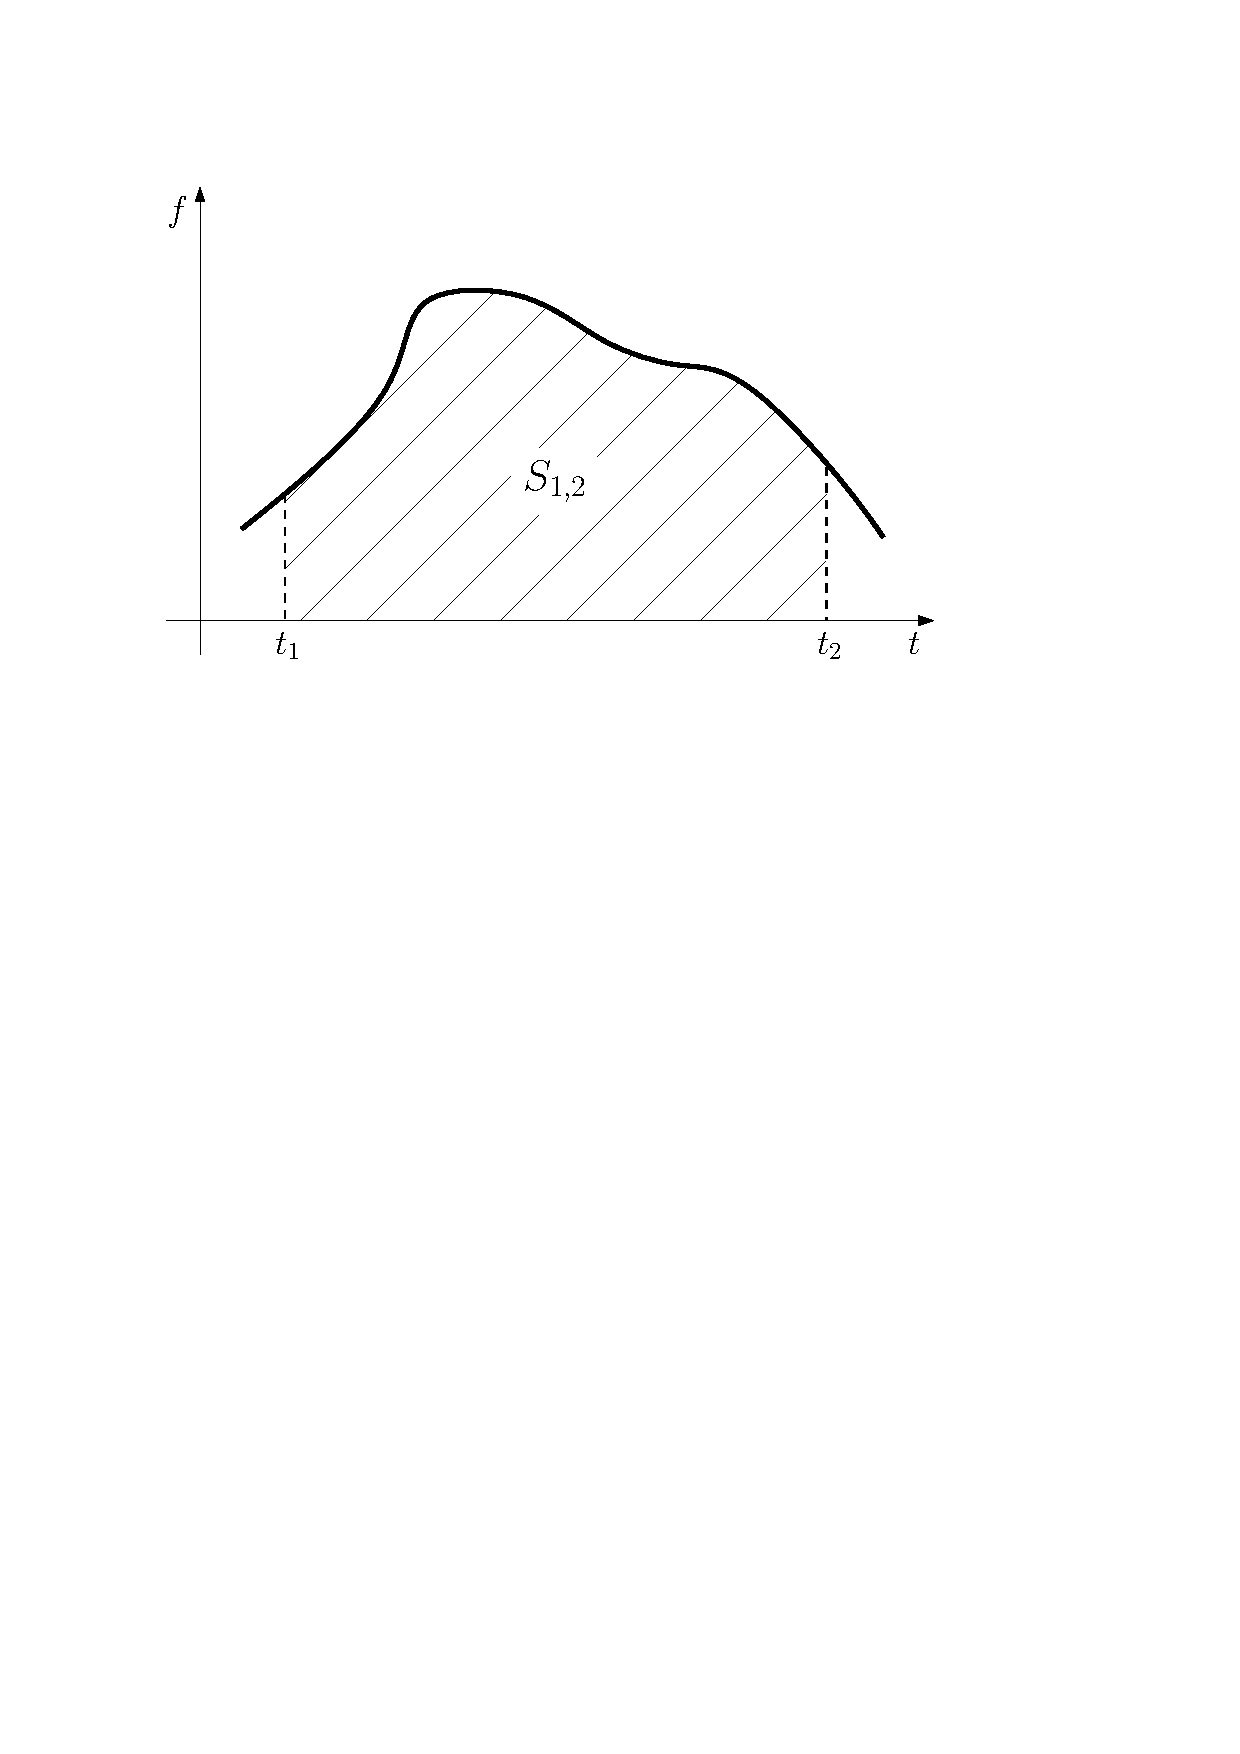
\includegraphics[width=0.6\textwidth]{geom_mean_integral.pdf} }
	\caption{Чертеж, поясняющий геометрический смысл определенного интеграла.}
	\label{fig:geom_mean_integral}
\end{figure}

\subsection{Метод правых прямоугольников}
\hspace*{\parindent}В~данном методе площадь под графиком интегрируемой функции оценивается по сумме площадей прямоугольников, показанных на рис.~\ref{fig:right_rect_method}.
Поиск значения определенного интеграла при этом ведется по следующим формулам:
\begin{align}
\int\limits_{t_m}^{t_{m+1}} f\,dt &\approx f_{m+1}(t_{m+1}-t_m), \quad m\in\mathbb{Z},\\
\int\limits_{t_m}^{t_{n}} f\,dt = \int\limits_{t_m}^{t_{m+1}} f\,dt + \int\limits_{t_{m+1}}^{t_{m+2}} f\,dt + \ldots &+ \int\limits_{t_{n-1}}^{t_{n}} f\,dt \approx f_{m+1}(t_{m+1}-t_m) + f_{m+2}(t_{m+2}-t_{m+1}) + \ldots + \notag\\
&+ f_{n}(t_{n}-t_{n-1}) = \sum\limits_{i=m+1}^{n}f_i(t_i-t_{i-1}), \quad m<n, \;\: m,n\in\mathbb{Z}\ldotp
\end{align}

\begin{figure}[p]
	\centering{ 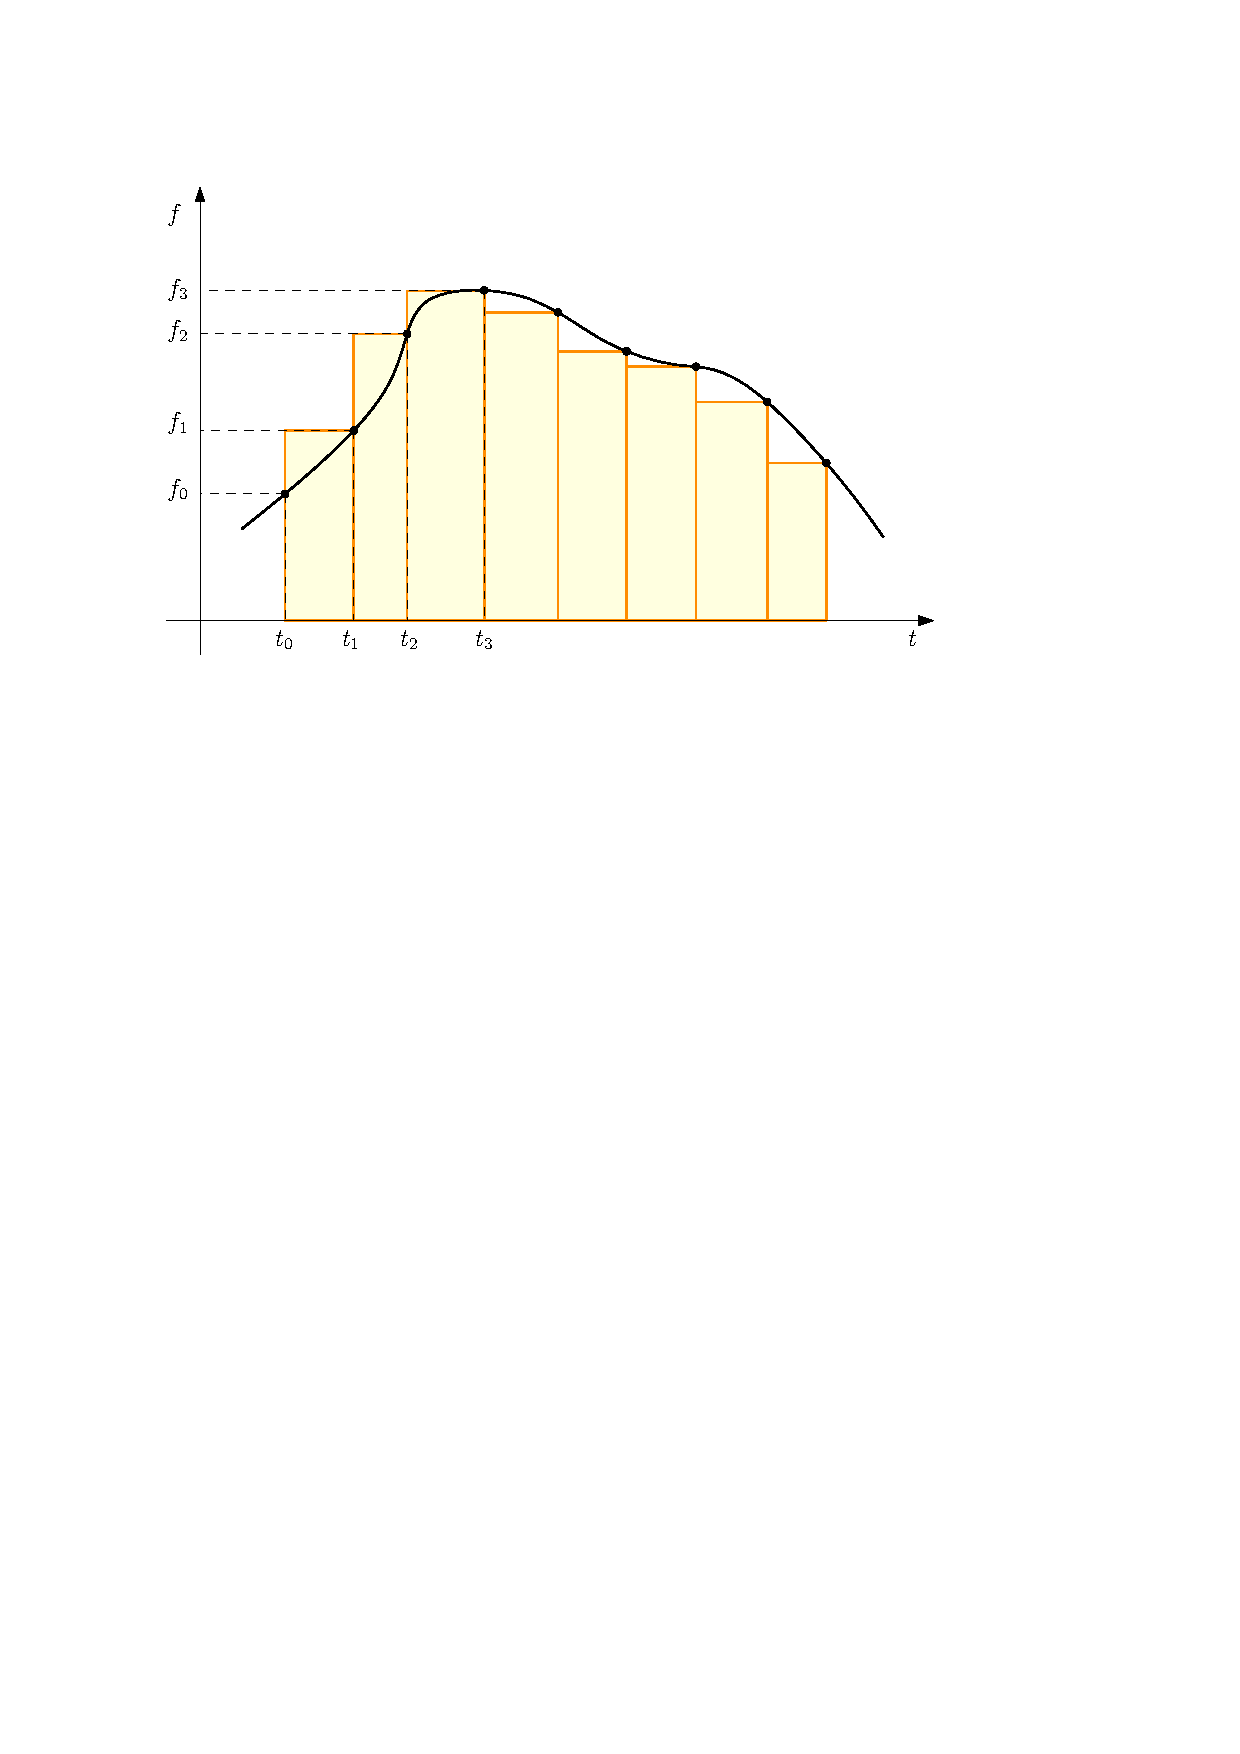
\includegraphics[width=0.65\textwidth]{right_rect_method.pdf} }
	\caption{Пояснение к вычислению определенного интеграла методом правых прямоугольников.}
	\label{fig:right_rect_method}
\end{figure}

\subsection{Метод левых прямоугольников}
\hspace*{\parindent}Этот метод практически идентичен прошлому и отличается от него только выбором используемых прямоугольников (см.~рис.~\ref{fig:left_rect_method}).
Формулы для этого случая также мало отличаются от выше приведенных:
\begin{align}
\int\limits_{t_m}^{t_{m+1}} f\,dt &\approx f_{m}(t_{m+1}-t_m), \quad m\in\mathbb{Z},\\
\int\limits_{t_m}^{t_{n}} f\,dt = \int\limits_{t_m}^{t_{m+1}} f\,dt + \int\limits_{t_{m+1}}^{t_{m+2}} f\,dt + \ldots &+ \int\limits_{t_{n-1}}^{t_{n}} f\,dt \approx f_{m}(t_{m+1}-t_m) + f_{m+1}(t_{m+2}-t_{m+1}) + \ldots + \notag\\
&+ f_{n-1}(t_{n}-t_{n-1}) = \sum\limits_{i=m}^{n-1}f_i(t_{i+1}-t_{i}), \quad m<n, \;\: m,n\in\mathbb{Z}\ldotp
\end{align}

\begin{figure}[p]
	\centering{ 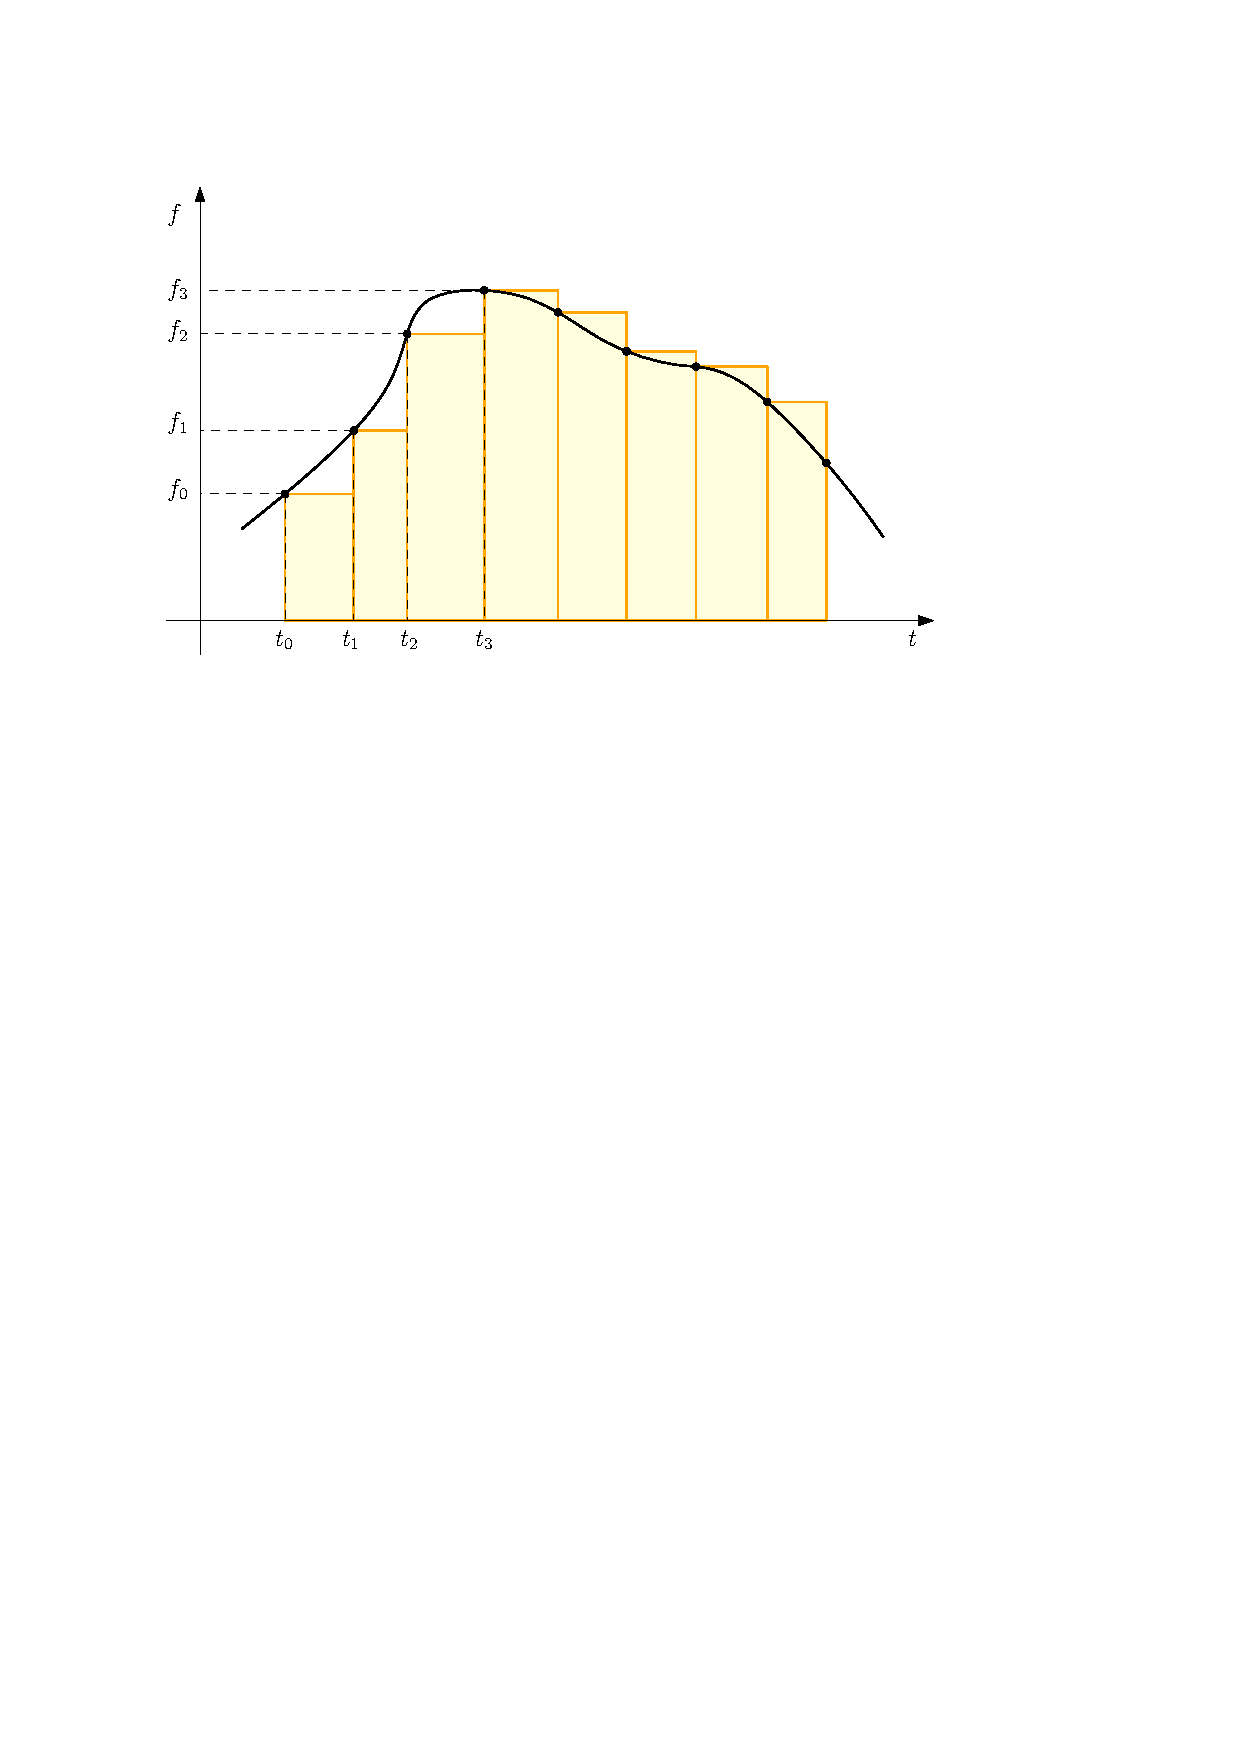
\includegraphics[width=0.65\textwidth]{left_rect_method.pdf} }
	\caption{Пояснение к вычислению определенного интеграла методом левых прямоугольников.}
	\label{fig:left_rect_method}
\end{figure}

\subsection{Метод средних прямоугольников}
\hspace*{\parindent}Для расчета значения определенного интеграла данным методом следует использовать суммы площадей прямоугольников, изображенных на рис.~\ref{fig:middle_rect_method}:
\begin{align}
\int\limits_{t_m}^{t_{m+2}} f\,dt &\approx f_{m+1}(t_{m+2}-t_m), \quad m\in\mathbb{Z},\\
\int\limits_{t_m}^{t_{n}} f\,dt = \int\limits_{t_m}^{t_{m+2}} f\,dt + \int\limits_{t_{m+2}}^{t_{m+4}} f\,dt + \ldots &+ \int\limits_{t_{n-2}}^{t_{n}} f\,dt \approx f_{m+1}(t_{m+2}-t_m) + f_{m+3}(t_{m+4}-t_{m+2}) + \ldots + \notag\\
+ f_{n-1}(t_{n}-t_{n-2}) &=\!\! \sum\limits_{\substack{i = m+1,\\i\ne m+2k}}^{n-1}\!\!f_i(t_{i+1}-t_{i-1}), \quad m<n, \;\: m,n\in\mathbb{Z}, \:\; k\in\mathbb{N}\ldotp
\end{align}

Свое название данный метод получил от следующего требования, предъявляемого к абсциссам используемых точек (записано с использованием обозначений, принятых на рис.~\ref{fig:middle_rect_method}):
\begin{equation}\label{eq:simm_requirement}
t_1 = \dfrac{t_0+t_2}{2}, \quad t_3 = \dfrac{t_2+t_4}{2}, \quad \ldots\quad\ldotp
\end{equation}

\begin{figure}[p]
	\centering{ 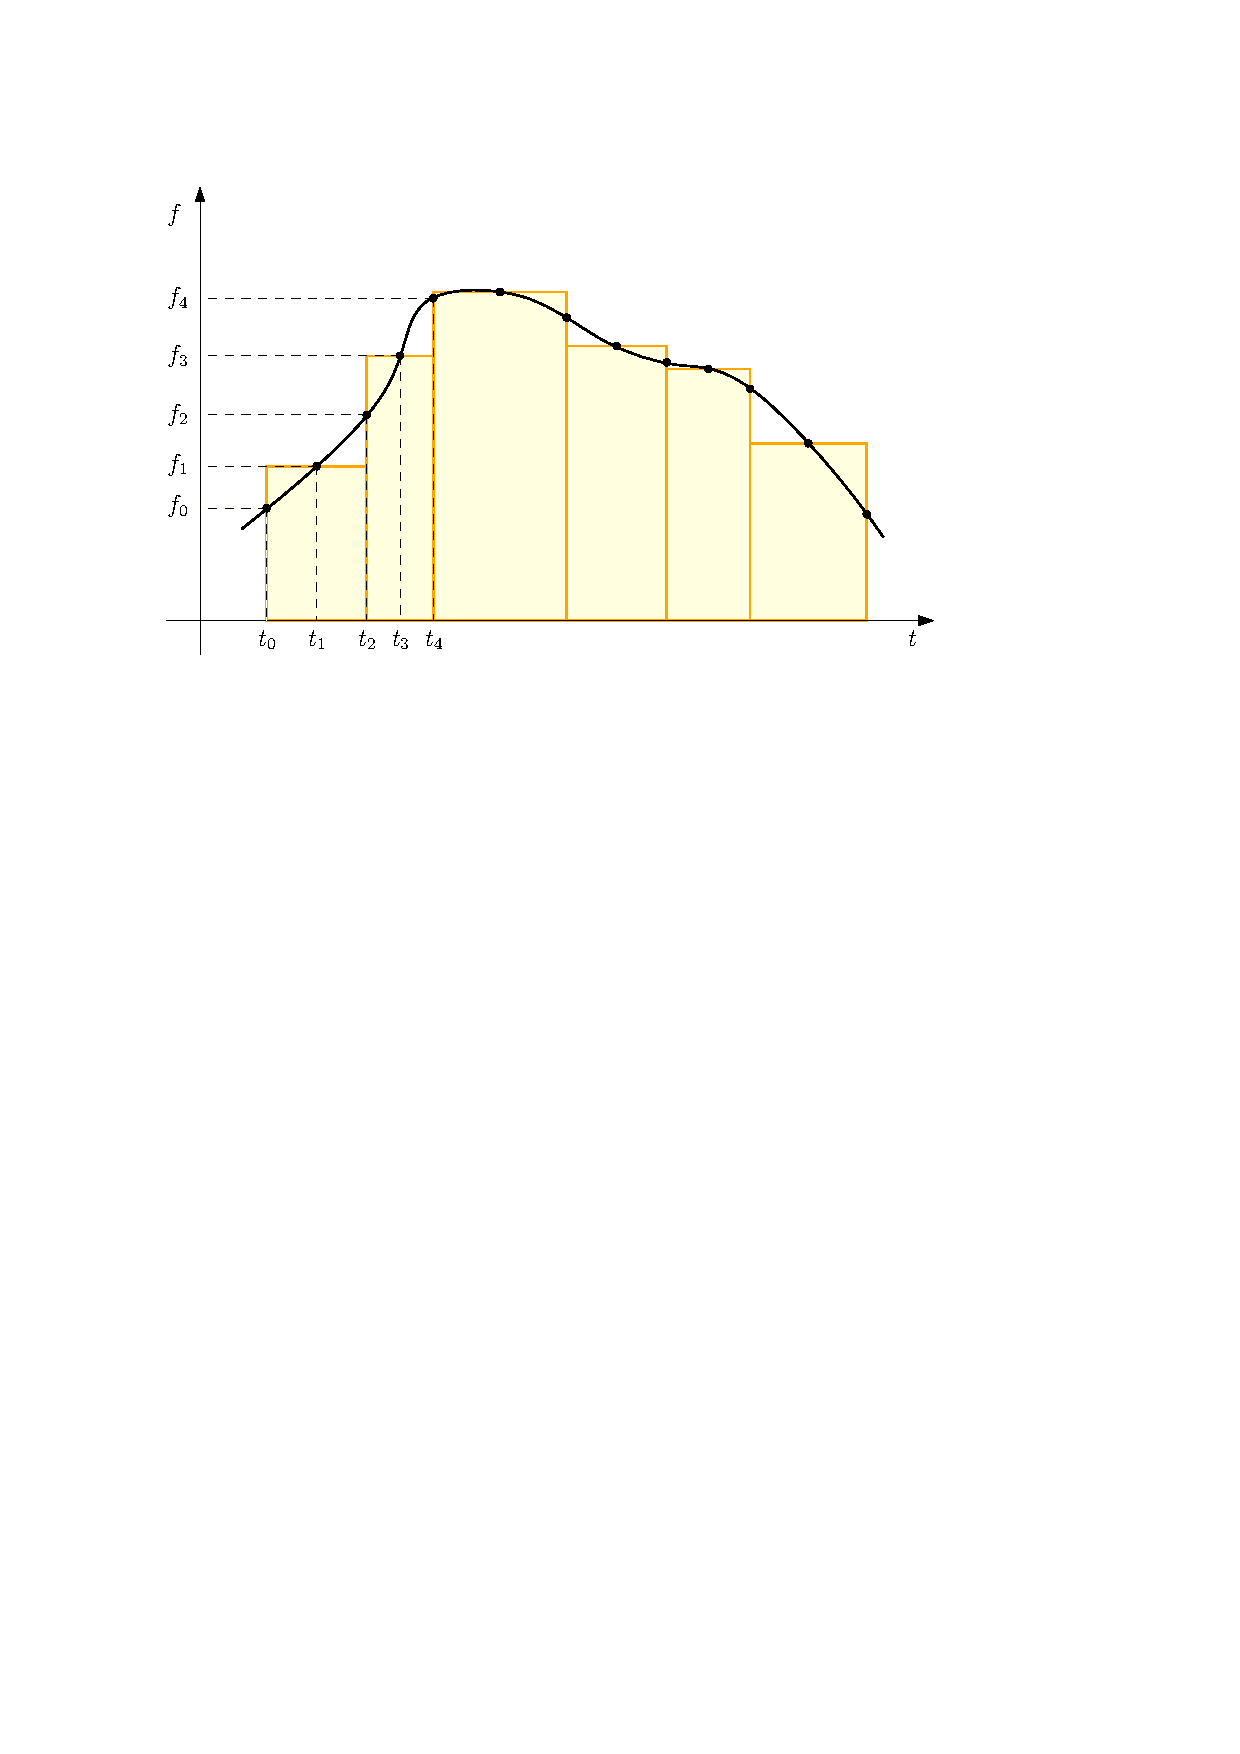
\includegraphics[width=0.65\textwidth]{middle_rect_method.pdf} }
	\caption{Пояснение к вычислению определенного интеграла методом средних прямоугольников.}
	\label{fig:middle_rect_method}
\end{figure}

\subsection{Метод трапеций}
\hspace*{\parindent}В~данном методе площадь под графиком рассматриваемой функции ищется как сумма площадей прямоугольных трапеций (см.~рис.~\ref{fig:trapezoid_method}).
Следовательно, для расчета значения определенного интеграла следует пользоваться формулами:
\begin{align}
\int\limits_{t_m}^{t_{m+1}} f\,dt \approx \dfrac{f_m+f_{m+1}}{2}&\cdot(t_{m+1}-t_m), \quad m\in\mathbb{Z}\\
\int\limits_{t_m}^{t_{n}} f\,dt = \int\limits_{t_m}^{t_{m+1}} f\,dt + \int\limits_{t_{m+1}}^{t_{m+2}} f\,dt + \ldots + \int\limits_{t_{n-1}}^{t_{n}} f\,dt &\approx  \dfrac{f_m+f_{m+1}}{2}\cdot(t_{m+1}-t_m) + \notag \\ + \dfrac{f_{m+1}+f_{m+2}}{2}\cdot(t_{m+2}-t_{m+1}) &+ \ldots + \dfrac{f_{n-1}+f_{n}}{2}\cdot(t_{n}-t_{n-1}) =\notag \\= \sum\limits_{i=m}^{n-1}&\dfrac{f_{i}+f_{i+1}}{2}\cdot(t_{i+1}-t_{i}), \quad m<n, \;\: m,n\in\mathbb{Z}
\end{align}

\begin{figure}[h!]
	\centering{ 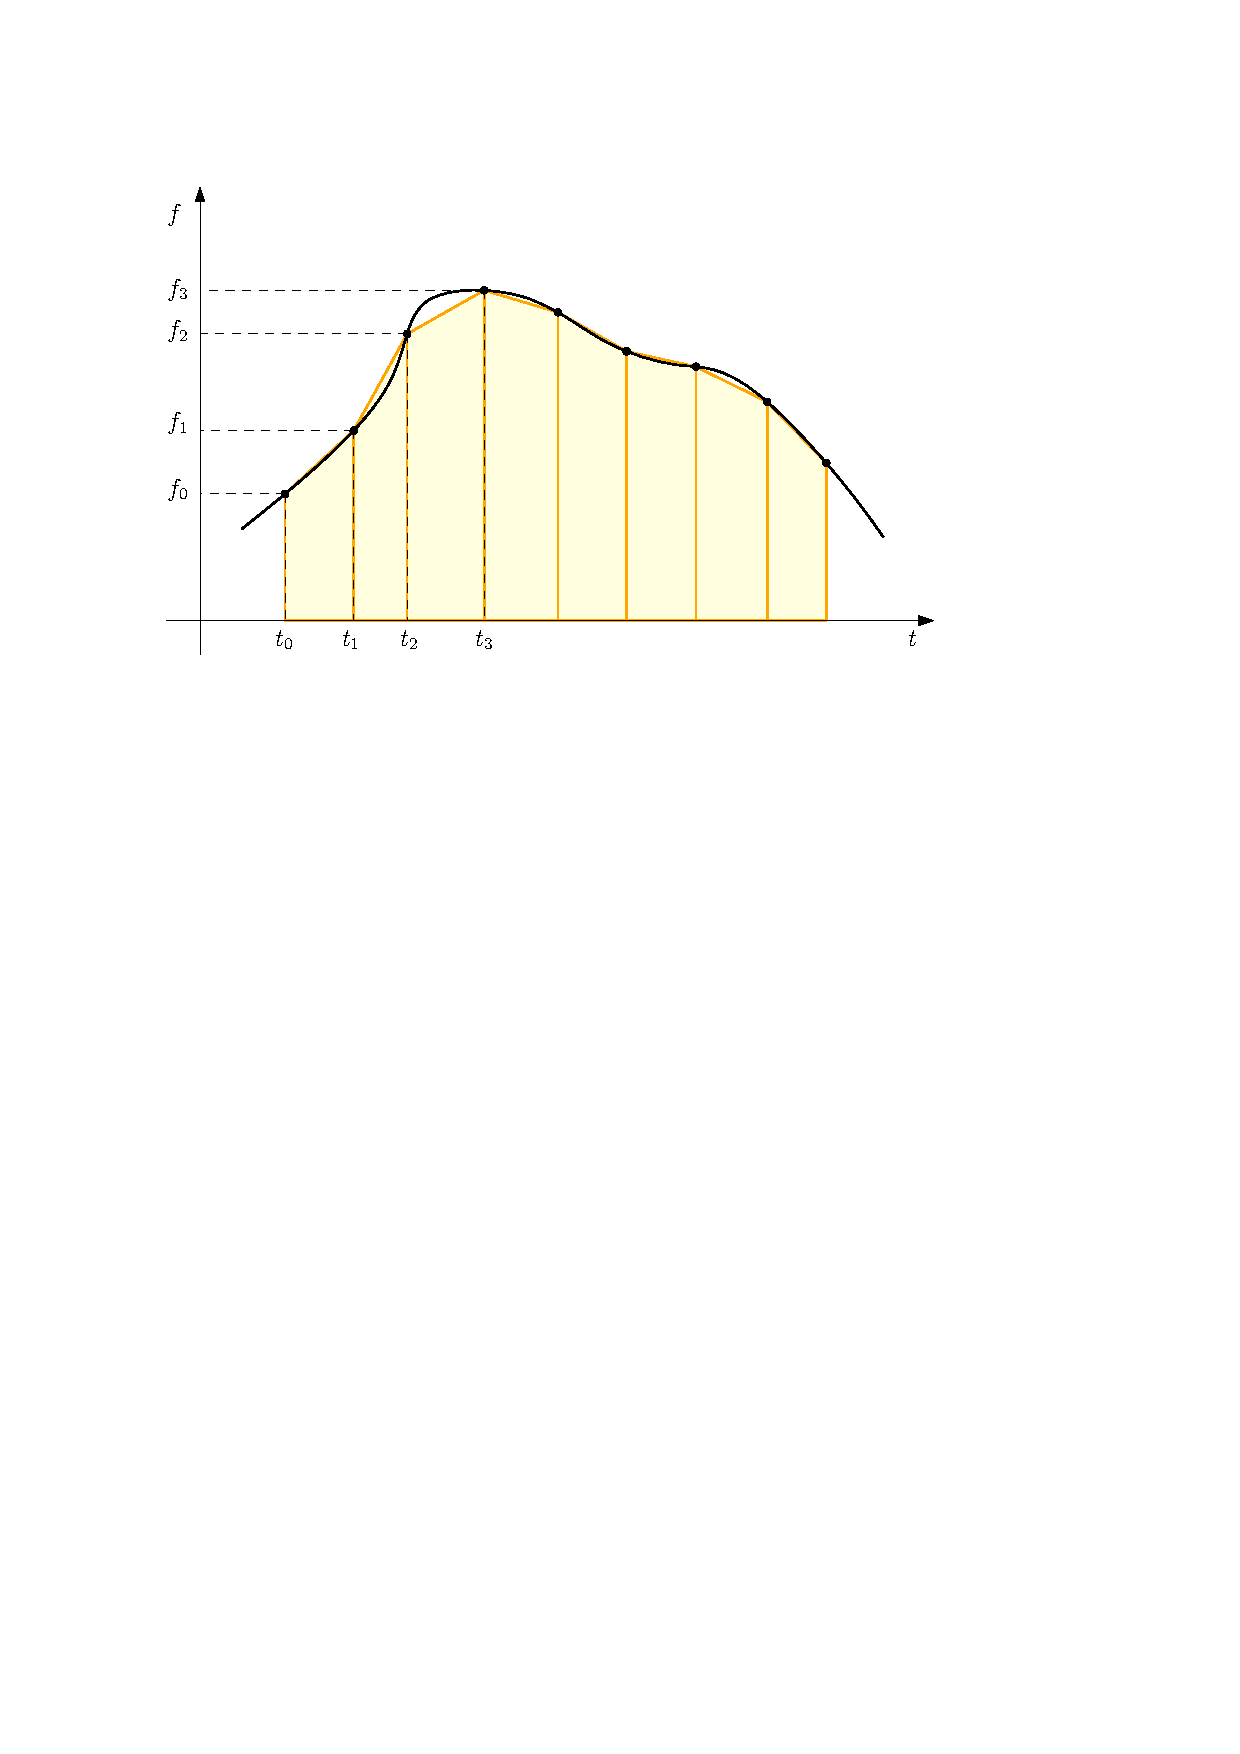
\includegraphics[width=0.65\textwidth]{trapezoid_method.pdf} }
	\caption{Пояснение к вычислению определенного интеграла методом трапеций.}
	\label{fig:trapezoid_method}
\end{figure}

\subsection{Метод парабол (Симпсона)}
\hspace*{\parindent}Через любые три точки с разными абсциссами на координатной плоскости проходит парабола и притом только одна (см.~рис.~\ref{fig:parabola_through_3_ponts}).
Справедливость данного утверждения можно продемонстрировать, например, следующим образом.

\begin{figure}[h!]
	\centering{ 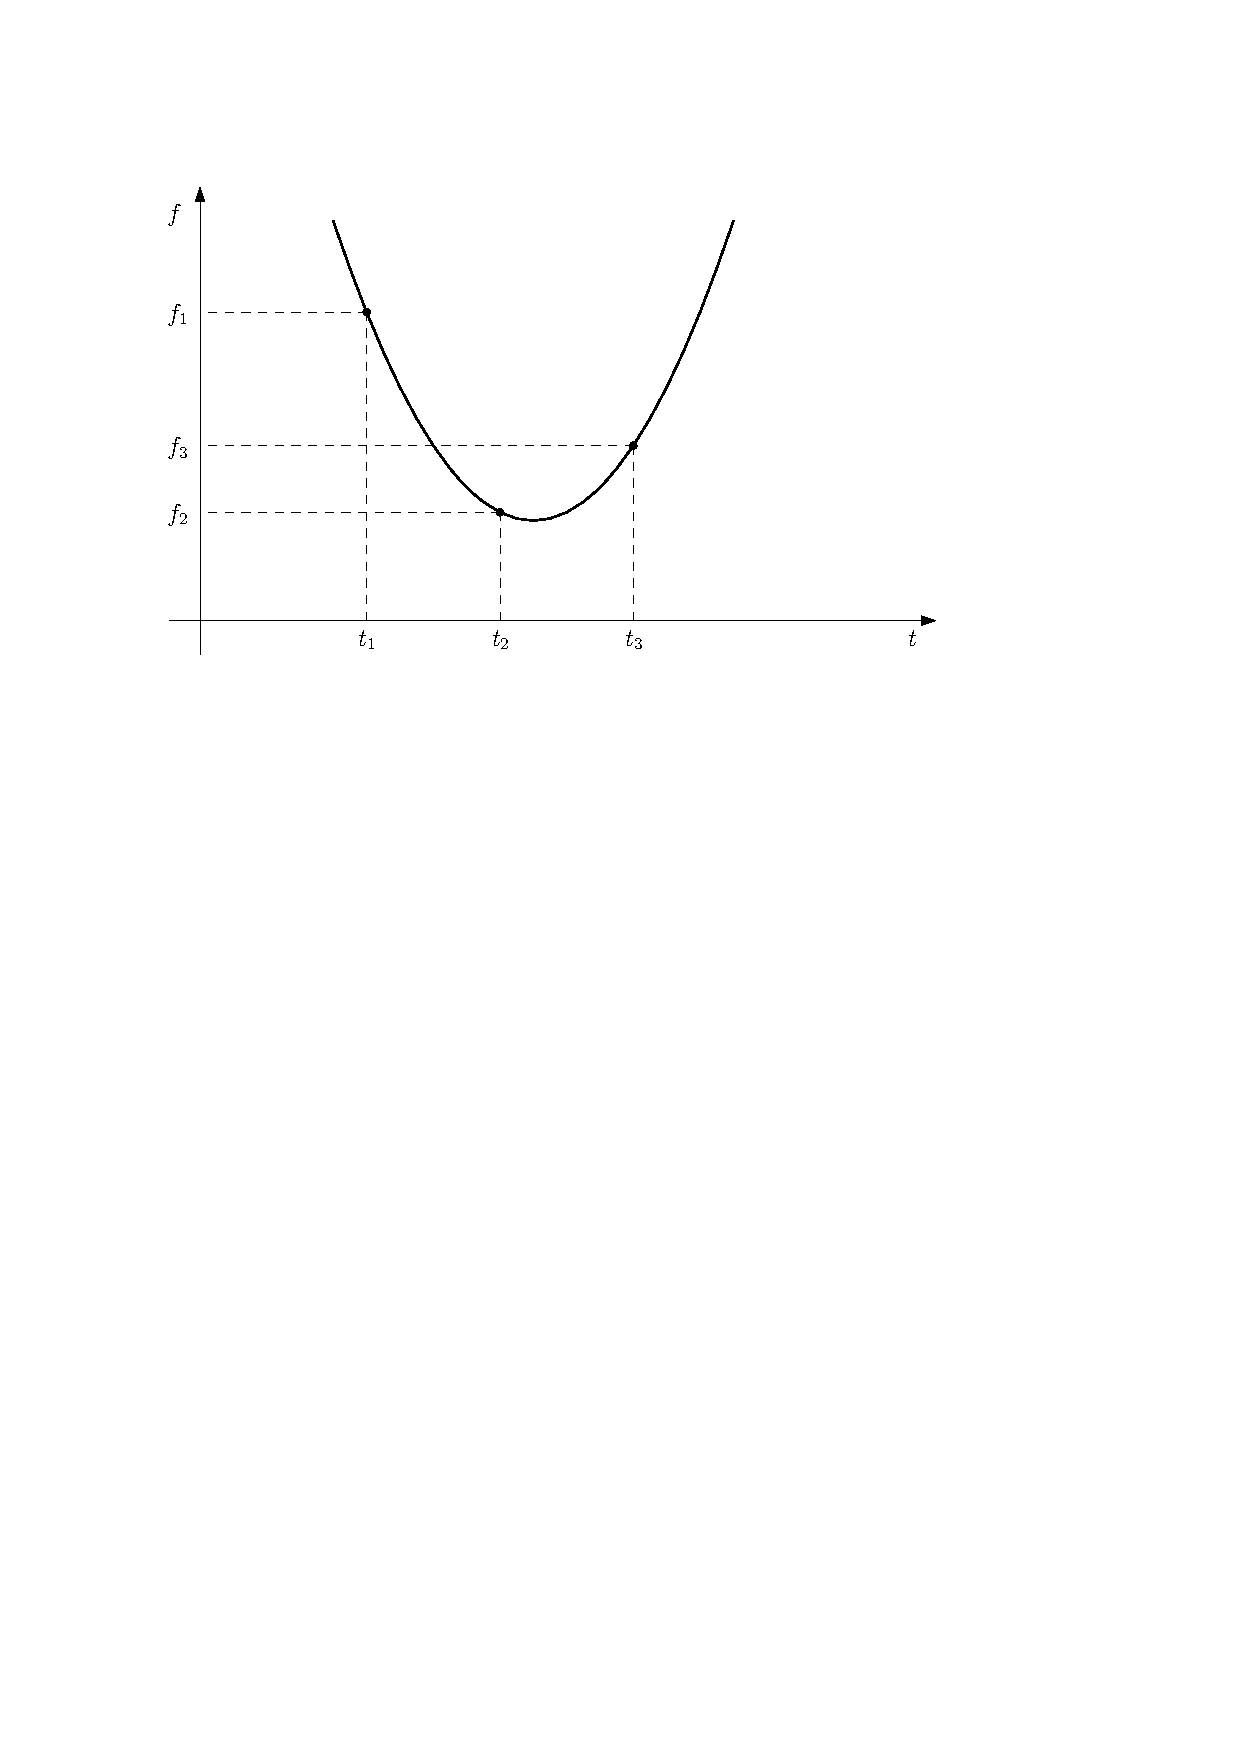
\includegraphics[width=0.65\textwidth]{parabola_through_3_ponts.pdf} }
	\caption{Пример параболы, проходящей через некоторые три точки.}
	\label{fig:parabola_through_3_ponts}
\end{figure}

Поставим себе задачу найти параметры $a$, $b$ и $c$ (см.~ниже) параболы, проходящей через заданные три точки с координатами $(t_1, f_1)$, $(t_2, f_2)$ и $(t_3, f_3)$.

Уже только из того факта, что парабола проходит через эти точки, оказываются справедливыми следующие три равенства:
\begin{equation}\label{eq:parabolas_in_point_eqs}
	\left\{  
	\begin{aligned}
		\!&a t_1^2 + b t_1 + c = f_1\\
		\!&a t_2^2 + b t_2 + c = f_2\\
		\!&a t_3^2 + b t_3 + c = f_3
	\end{aligned}   
	\right.
\end{equation}
В~матричном виде они могут быть переписаны, как:
\begin{equation}
\begin{bmatrix}
t_1^2 & t_1 & 1\\
t_2^2 & t_2 & 1\\
t_3^2 & t_3 & 1
\end{bmatrix}
\begin{bmatrix}
a \\ b \\ c
\end{bmatrix}
=
\begin{bmatrix}
f_1 \\ f_2 \\ f_3
\end{bmatrix}
\end{equation}
Из этого выражения для неизвестных параметров можно получить следующую расчетную формулу:
\begin{equation}\label{eq:a_b_c_finder}
\begin{bmatrix}
a \\ b \\ c
\end{bmatrix}
=
\begin{bmatrix}
t_1^2 & t_1 & 1\\
t_2^2 & t_2 & 1\\
t_3^2 & t_3 & 1
\end{bmatrix}^{-1}\cdot
\begin{bmatrix}
f_1 \\ f_2 \\ f_3
\end{bmatrix}
\end{equation}

Определитель матрицы, содержащей значения абсцисс точек, равен:
\begin{multline}
\begin{vmatrix}
t_1^2 & t_1 & 1\\
t_2^2 & t_2 & 1\\
t_3^2 & t_3 & 1
\end{vmatrix} = t_2^2 t_3 - t_2 t_3^2 - t_1^2 t_3 + t_1 t_3^2 + t_1^2 t_2 - t_1 t_2^2 = \underline{\underline{t_2^2 t_3}} - \underline{\underline{t_2 t_3^2}} - \underline{t_1^2 t_3} + \underline{t_1 t_3^2} + \underline{t_1^2 t_2} - \underline{\underline{t_1 t_2^2}} +\\
%
+\underline{\underline{t_1 t_2 t_3}} - \underline{t_1 t_2 t_3}  = t_1(-t_1 t_3 + t_3^2 + t_1 t_2 - t_2 t_3) - t_2(-t_2 t_3 + t_3^2 + t_1 t_2 -t_1 t_3) = \\
%
= (t_1-t_2)(-t_1 t_3 + t_3^2 + t_1 t_2 - t_2 t_3) = (t_1 - t_2)(t_3 - t_1)(t_3 - t_2)
\end{multline}
и, следовательно, при условии, что абсциссы $t_1$, $t_2$ и $t_3$ не равны друг другу, отличен от нуля.
Это свойство в свою очередь позволяет заключить, что обратная матрица в выражении~\eqref{eq:a_b_c_finder} существует.
Значит, относительно параметров $a$, $b$ и $c$ это уравнение разрешимо единственным образом.
Значит, через эти три точки действительно проходит парабола и при этом только одна.~$\blacksquare$

Метод парабол (метод Симпсона) основывается на данном свойстве и приближает искомый определенный интеграл суммой площадей криволинейных трапеций, формируемых параболами, проходящими через точки интегрируемой функции (см.~рис.~\ref{fig:parabolas_method}).
Расчетные формулы при этом выглядят следующим образом:
\begin{equation}\label{eq:square_of_1_parabola}
\int\limits_{t_m}^{t_{m+2}} f\,dt \approx \dfrac{t_{m+2} - t_{m}}{6}(f_m + 4f_{m+1} + f_{m+2}), \quad m\in\mathbb{Z},
\end{equation}
\vspace{-0.5cm}
\begin{multline}
\int\limits_{t_m}^{t_{n}} f\,dt = \int\limits_{t_m}^{t_{m+2}} f\,dt + \int\limits_{t_{m+2}}^{t_{m+4}} f\,dt + \ldots + \int\limits_{t_{n-2}}^{t_{n}} f\,dt \approx \dfrac{t_{m+2} - t_{m}}{6}(f_m + 4f_{m+1} + f_{m+2}) +\\
%
+ \dfrac{t_{m+4} - t_{m+2}}{6}(f_{m+2} + 4f_{m+3} + f_{m+4}) + \ldots + \dfrac{t_{n} - t_{n-2}}{6}(f_{n-2} + 4f_{n-1} + f_{n}) =\\
%
=\!\! \sum\limits_{\substack{i = m+1,\\i\ne m+2k}}^{n-1}\!\!\dfrac{t_{i+1} - t_{i-1}}{6}(f_{i-1} + 4f_{i} + f_{i+1}), \quad m<n, \;\: m,n\in\mathbb{Z}, \:\; k\in\mathbb{N}\ldotp
\end{multline}

Следует отметить, что эти формулы справедливы только при условии, аналогичном~\eqref{eq:simm_requirement}.
Другими словами, значение абсциссы каждой второй точки из всех участвующих в интегрировании должно быть средним арифметическим значений абсцисс соседних с ней точек.

\begin{figure}[h!]
	\centering{ 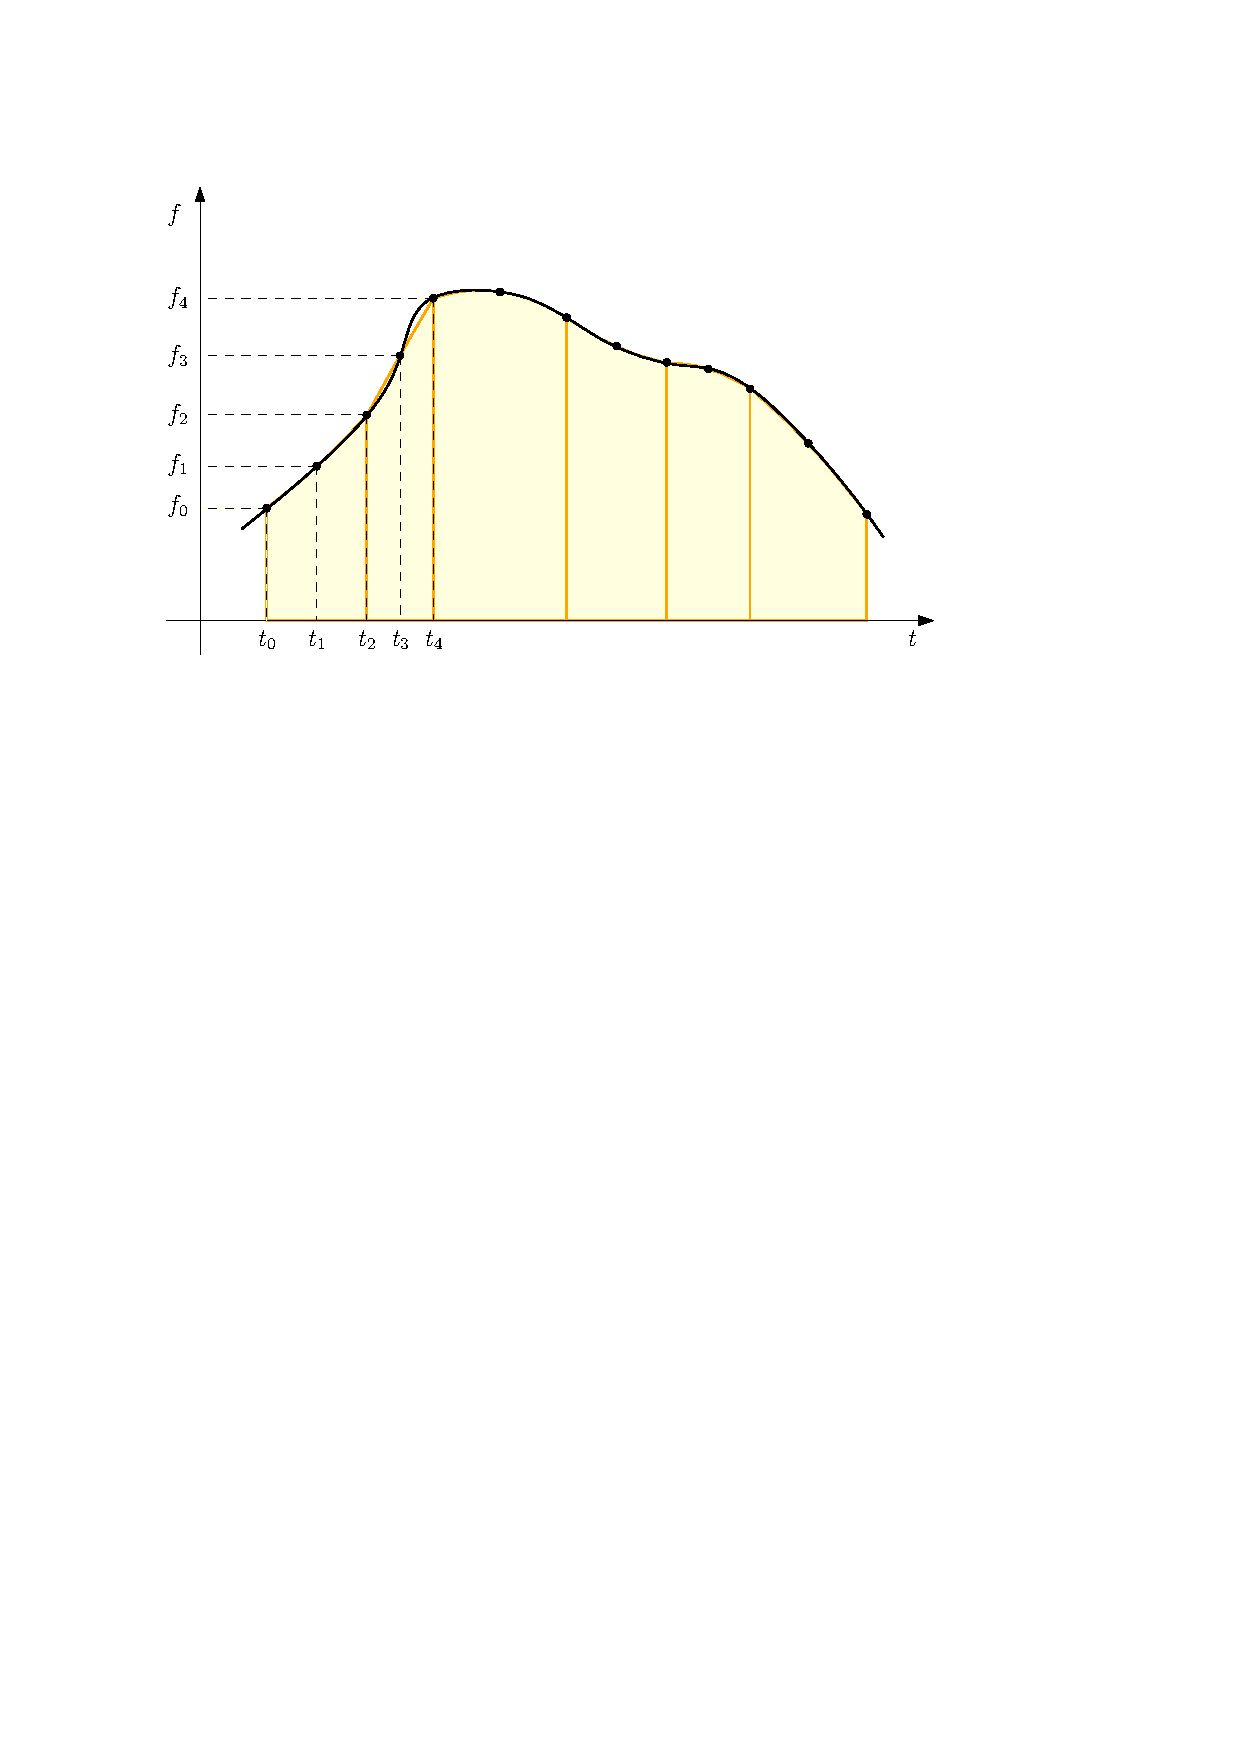
\includegraphics[width=0.65\textwidth]{parabolas_method.pdf} }
	\caption{Пояснение к вычислению определенного интеграла методом парабол.}
	\label{fig:parabolas_method}
\end{figure}

Поскольку правая часть выражения~\eqref{eq:square_of_1_parabola}, представляющая собой формулу для площади криволинейной трапеции, ограниченной сверху параболой, далеко не очевидна, докажем ее.

Рассмотрим чертеж, изображенный на рис.~\ref{fig:parabola_through_3_ponts}, и ситуацию, при которой 
\begin{equation}\label{eq:h_was_born_here}
t_3-t_2 = t_2-t_1 = h\ldotp
\end{equation}

Из выражений~\eqref{eq:parabolas_in_point_eqs} и~\eqref{eq:h_was_born_here} следует, что
\begin{gather}
f_1 = a t_1^2 + b t_1 + c = a (t_2 - h)^2 + b(t_2 -h) + c = a t_2^2 - 2a h t_2 + a h^2 + b t_2 - b h + c,\label{eq:f1_super_eqs}\\
%
f_3 = a t_3^2 + b t_3 + c = a (t_2 + h)^2 + b(t_2 + h) + c = a t_2^2 + 2a h t_2 + a h^2 + b t_2 + b h + c,\\
%
f_3 - f_1 = 4 a h t_2 + 2 b h\ldotp \label{eq:f3mf1_super_eqs}
\end{gather}

Рассматриваемый интеграл с учетом выражений~\eqref{eq:f1_super_eqs}--\eqref{eq:f3mf1_super_eqs} равен:
\begin{multline}
\int\limits_{t_1}^{t_{3}} f\,dt = \int\limits_{t_1}^{t_{3}} \left(at^2+bt+c\right)\,dt = \left.\left(\dfrac{at^3}{3} + \dfrac{bt^2}{2}+ct\right)\right|^{t_3}_{t_1} = \frac{1}{6}\left(2at_3^3 + 3bt_3^2 + 6ct_3 - 2at_1^3 -\right.\\
%
\left.- 3bt_1^2 - 6ct_1\right) = \frac{1}{6}\left(2at_3^3 + 2bt_3^2 + 2ct_3 + bt_3^2 + 4ct_3 - 2at_3^3 - 2bt_3^2 - 2ct_3 - bt_3^2 - 4ct_3\right) =\\
%
= \frac{1}{6}\left(2t_3f_3 + bt_3^2 + 4ct_3 - 2t_1f_1 - bt_1^2 - 4ct_1\right) = \frac{1}{6}\left(2(t_2+h)f_3 + b(t_2+h)^2 + 4c(t_2+h) -\right.\\
%
\left.- 2(t_2-h)f_1 - b(t_2-h)^2 - 4c(t_2-h)\right) = \frac{1}{6}\left(2t_2(f_3-f_1) + 2h(f_3+f_1) + 4hbt_2 + 8hc\right) = \\
%
=\frac{1}{6}\left(2t_2(4aht_2 + 2bh) + 2h(f_3+f_1) + 4hbt_2 + 8hc\right) = \frac{1}{6}\left(2h(f_3+f_1)+8hat_2^2 + 8hbt_2+\right.\\
%
+ 8hc\bigr)=\frac{1}{6}\left(2h(f_3+f_1)+2h(4at_2^2 + 4bt_2 + 4c)\right) = \frac{h}{3}\left(f_1+4f_2+f_3\right)\ldotp
\end{multline}
Получившееся выражение с учетом~\eqref{eq:h_was_born_here} совпадает с~\eqref{eq:square_of_1_parabola}.~$\blacksquare$

\section{Численное дифференцирование}
\hspace*{\parindent}Производная функции в данной в точке равна угловому коэффициенту касательной, проведенной к графику функции в этой точке (см.~рис.~\ref{fig:derivative_calc}):
\begin{equation}
f'(t_1) = \lim_{\Delta t\rightarrow 0} \dfrac{f(t_1+\Delta t) - f(t_1)}{\Delta t} = \tg\varphi
\end{equation}

\begin{figure}[h!]
	\centering{ 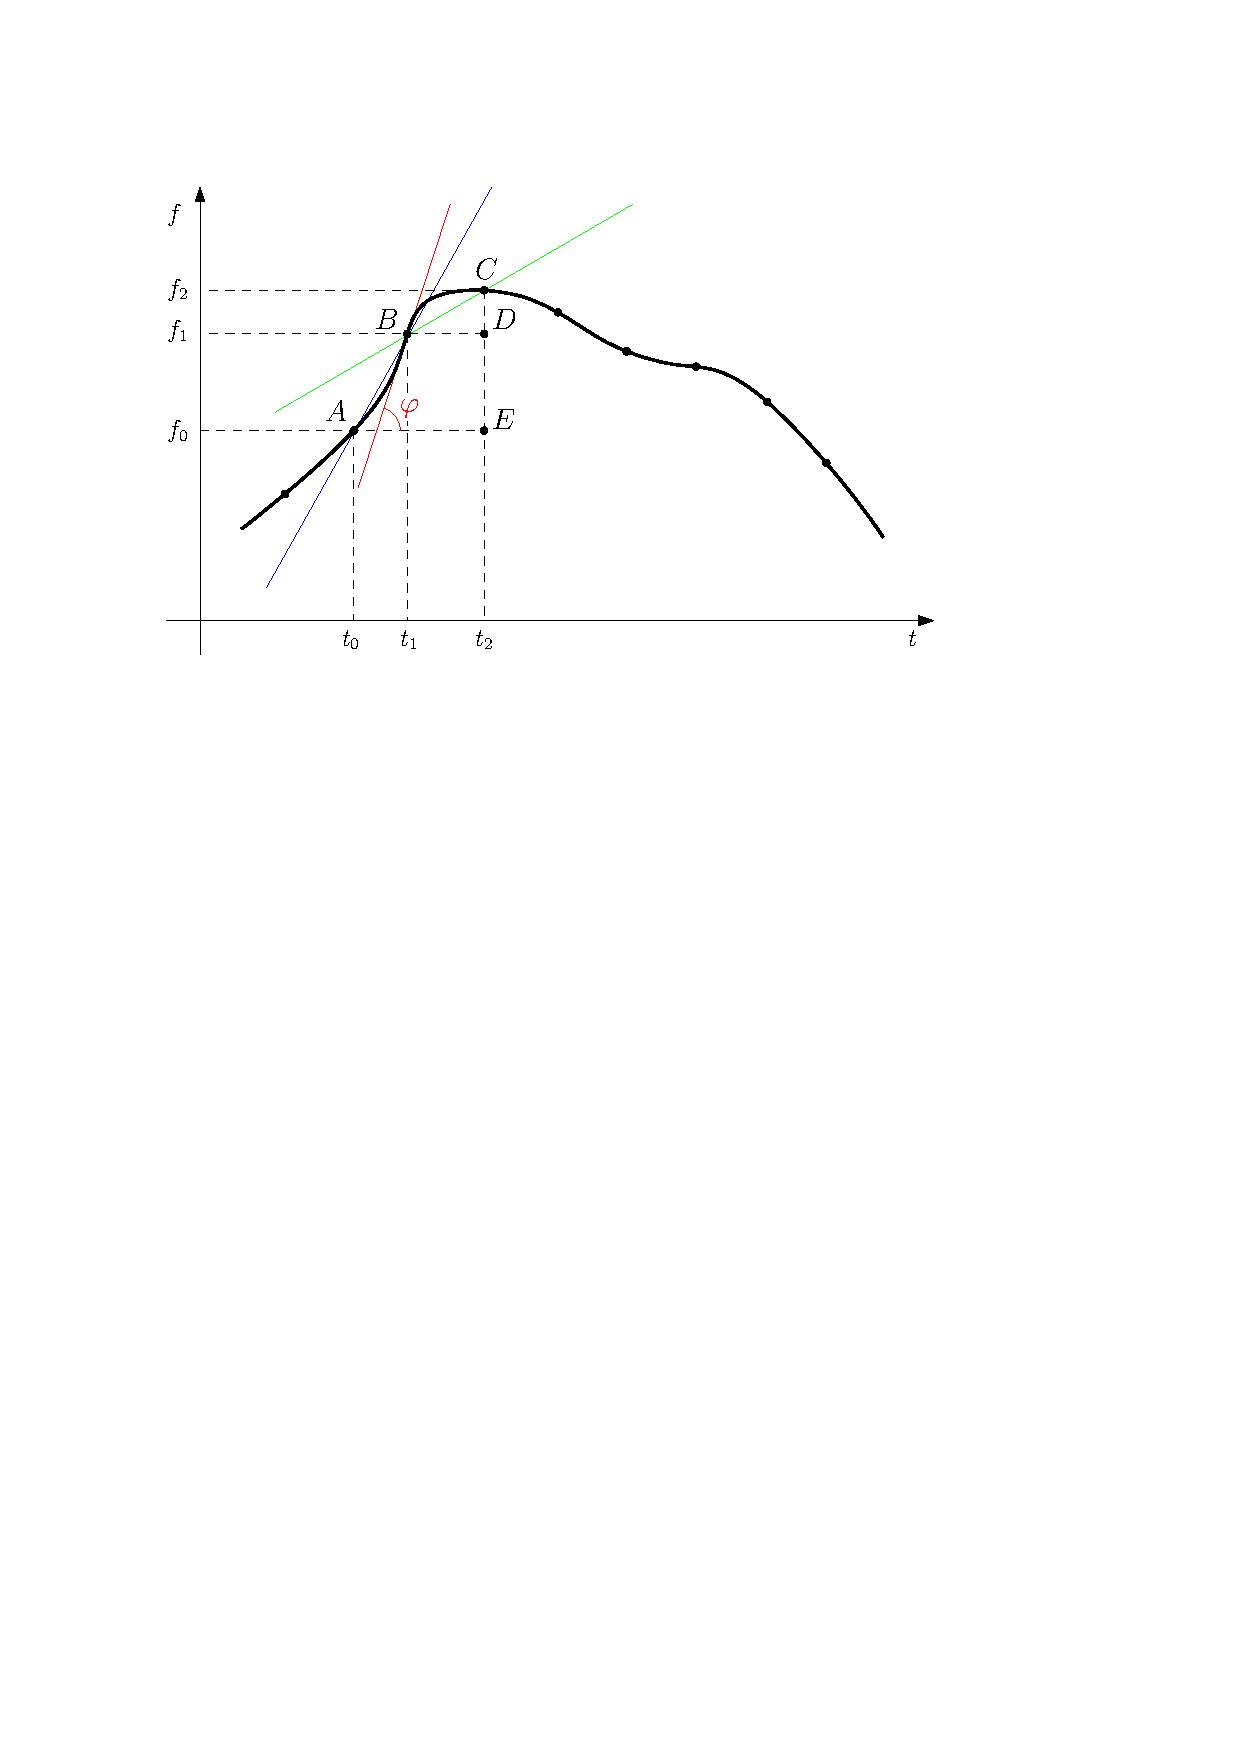
\includegraphics[width=0.65\textwidth]{derivative_calc.pdf} }
	\caption{Пояснение к вычислению значения производной функции в точке.}
	\label{fig:derivative_calc}
\end{figure}


Метод приближенного расчета этого значения через тангенс угла наклона секущей, проходящей через точки $B$ и $C$:
\begin{equation}
f'(t_1) \approx \dfrac{f_2-f_1}{t_2-t_1} = \tg\angle CBD
\end{equation}
называется \textit{методом правосторонней разности}, а через тангенс угла наклона секущей, проходящей через точки $A$ и $B$:
\begin{equation}
f'(t_1) \approx \dfrac{f_1-f_0}{t_1-t_0} = \tg\angle BAE
\end{equation}
--- 	\textit{методом левосторонней разности}.

Если для абсцисс используемых точек выполняются следующие равенства:
\begin{equation}
t_2 - t_1 = t_1 - t_0 = h,
\end{equation}
то значение производной можно рассчитать точнее, найдя среднее арифметическое оценок, получаемых в результате использования двух предыдущих методов:
\begin{equation}
f'(t_1) \approx \frac{1}{2}\left(\dfrac{f_2-f_1}{t_2-t_1} + \dfrac{f_1-f_0}{t_1-t_0}\right) = \dfrac{f_2-f_0}{2h}\ldotp
\end{equation}
Такая схема приближенного расчета значения $f'(t_1)$ называется \textit{методом двусторонней разности}.
\end{document}